\chapter{Tautocrona}
Possiamo vedere il pendolo come un punto che scorre su una guida circolare liscia soggetto alla forza peso

La frequenza di oscillazione del pendolo è dipendente dai dati iniziali ovvero dall'energia.

Ci domandiamo se esiste una curva non circolare che assicura una frequenza di oscillazione indipendente dai dati iniziali. Questa curva è una cicloide ribaltata. Costruiamo una sua parametrizzazione. La cicloide è la traiettoria percorsa da un punto sul bordo di un disco che si muove di puro rotolamento. Prendiamo un disco che rotola di raggio \(R\)

\[
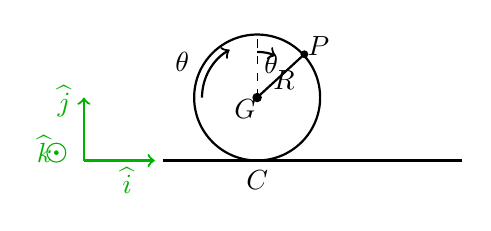
\begin{tikzpicture}
  \draw[green!70!black, thick, ->] (-2.2,0) -- (-2.2,0.8);
  \node[green!70!black] at (-2.45,0.75) {\(\widehat{j}\)};
  \draw[green!70!black, thick, ->] (-2.2,0) -- (-1.3,0);
  \node[green!70!black] at (-1.65,-0.25) {\(\widehat{i}\)};
  \node[green!70!black] at (-2.7,0.15) {\(\widehat{k}\)};
  \draw[green!70!black] (-2.55,0.1) circle (0.12);
  \fill[green!70!black] (-2.55,0.1) circle (0.03);

  \draw[thick] (-1.2,0) -- (2.6,0);
  \draw[thick] (0,0.8) circle (0.8);
  \filldraw[black] (0,0.8) circle (1.5pt);
  \node at (-0.15,0.65) {\(G\)};
  \node at (0,-0.25) {\(C\)};

  \draw[dashed] (0,0.8) -- (0,1.6);
  \draw[thick] (0,0.8) -- (0.6,1.35);
  \filldraw[black] (0.6,1.35) circle (1.2pt);
  \node at (0.78,1.45) {\(P\)};
  \node at (0.34,1.02) {\(R\)};

  \draw[thick, ->] (-0.7,0.8) arc (180:120:0.7);
  \node at (-0.95,1.25) {\(\theta\)};
  \draw[thick, ->] (0,1.38) arc (90:66:0.58);
  \node at (0.18,1.23) {\(\theta\)};
\end{tikzpicture}
\]

\[
\underline{v}_G = R\dot{\theta}\,\widehat{i}
\qquad
\underline{v}_P =
\underline{v}_G + \omega \wedge (\underline{x}_P-\underline{x}_G)
=
R\dot{\theta}\,\widehat{i}
-
\dot{\theta}\widehat{k}\wedge
\left(R\sin\theta\,\widehat{i}+R\cos\theta\,\widehat{j}\right)
=
\]
\[
=
R\dot{\theta}\,\widehat{i}
+
R\dot{\theta}\cos\theta\,\widehat{i}
-
R\dot{\theta}\sin\theta\,\widehat{j}
\]

Integriamo ponendo \(\theta(0)=\theta_0\).

\[
\dot{x}_P = R\dot{\theta}(1+\cos\theta)
\Rightarrow
\int_0^t \dot{x}_P\,dt
=
R\int_0^t \dot{\theta}+\dot{\theta}(\cos\theta)\,dt
\Rightarrow
x_P(t)=R(\theta-\theta_0)+R\sin\theta-R\sin\theta_0
\]

\[
\dot{y}_P=-R\dot{\theta}\sin\theta
\Rightarrow
\int_0^t \dot{y}_P\,dt
=
\int_0^t -R\dot{\theta}\sin\theta\,dt
\Rightarrow
y_P(t)=R\cos\theta-R\cos\theta_0
\]

\[
\Rightarrow
\underline{x}_P(t)
=
\left(R(\theta+\sin\theta)-R(\theta_0+\sin\theta_0)\right)\widehat{i}
+
\left(R\cos\theta-R\cos\theta_0\right)\widehat{j}
\]

\[
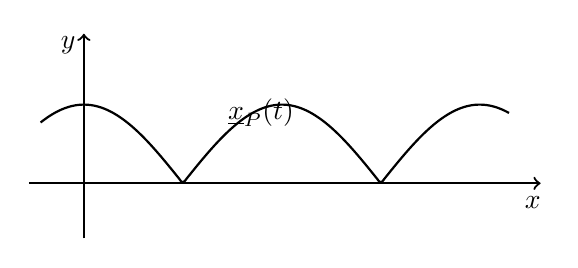
\begin{tikzpicture}
  \draw[thick, ->] (0,-0.7) -- (0,1.9);
  \node at (-0.2,1.75) {\(y\)};
  \draw[thick, ->] (-0.7,0) -- (5.8,0);
  \node at (5.7,-0.25) {\(x\)};
  \draw[thick, domain=-0.55:5.4, samples=200, smooth]
    plot ({\x},{abs(cos(1.25*\x r))});
  \node at (2.25,0.9) {\(\underline{x}_P(t)\)};
\end{tikzpicture}
\]

Rovesciamo la curva
\[
\widetilde{\underline{x}}_P(t)
=
R(\theta+\sin\theta)\widehat{i}
-
R\cos\theta\,\widehat{j}
-
R(\theta_0+\sin\theta_0)\widehat{i}
+
R\cos\theta_0\,\widehat{j}
=
\]
\[
=
R(\theta+\sin\theta)\widehat{i}
-
R\cos\theta\,\widehat{j}
+
\underline{K},
\qquad
\underline{K}\in\mathbb{R}^2
\]

\[
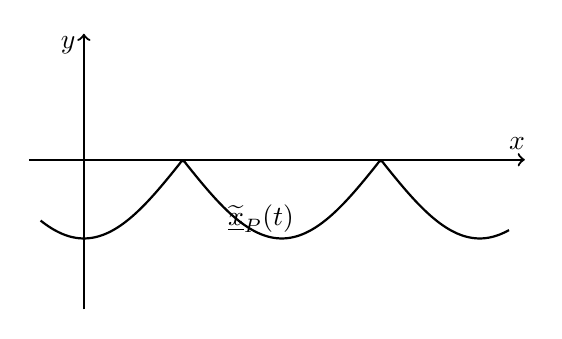
\begin{tikzpicture}
  \draw[thick, ->] (0,-1.9) -- (0,1.6);
  \node at (-0.2,1.45) {\(y\)};
  \draw[thick, ->] (-0.7,0) -- (5.6,0);
  \node at (5.5,0.2) {\(x\)};
  \draw[thick, domain=-0.55:5.4, samples=200, smooth]
    plot ({\x},{-abs(cos(1.25*\x r))});
  \node at (2.25,-0.75) {\(\widetilde{\underline{x}}_P(t)\)};
\end{tikzpicture}
\]

Studio il moto di un punto nella cicloide rovesciata.

Il potenziale è
\[
V=-mgR\cos\theta+K_2
\]

Scriviamo l'energia cinetica

\[
\widetilde{\underline{v}}_P
=
R\dot{\theta}\,\widehat{i}
+
R\cos\theta\,\dot{\theta}\,\widehat{i}
+
R\dot{\theta}\sin\theta\,\widehat{j}
\Rightarrow
T=
\frac{1}{2}m\widetilde{v}_P^2
=
\left[
\left(R\dot{\theta}+R\dot{\theta}\cos\theta\right)^2
+
\left(R\dot{\theta}\sin\theta\right)^2
\right]\frac{m}{2}
=
\]
\[
=
\frac{m}{2}R^2\dot{\theta}^2
\left[
(1+\cos\theta)^2+\sin^2\theta
\right]
=
\frac{m}{2}R^2\dot{\theta}^2
\left[
2+2\cos\theta
\right]
=
mR^2\dot{\theta}^2(1+\cos\theta)
\]

\[
\mathcal{L}
=
mR^2\dot{\theta}^2(1+\cos\theta)
+
mgR\cos\theta
-
K_2
\qquad
E=
mR^2\dot{\theta}^2(1+\cos\theta)
-
mgR\cos\theta
+
K_2
\]

Ipotizzo anche \(\dot{\theta}(0)=0\). Allora

\[
E(t)=E(0)
=
mR^2\dot{\theta}^2(1+\cos\theta)
-
mgR\cos\theta
=
+K_2
-
mgR\cos\theta_0
\]

Pongo convenzionalmente \(K_2=0\)

\[
mR^2\dot{\theta}^2(1+\cos\theta)
=
mgR(\cos\theta-\cos\theta_0)
\]

Il fatto che \(\cos\theta-\cos\theta_0\ge 0 \Leftrightarrow \cos\theta\ge\cos\theta_0 \Rightarrow \theta\le\theta_0\) è coerente con il senso fisico perché se il corpo parte con velocità nulla tenderà ad invertire il suo angolo di rotazione.

\[
\dot{\theta}^2
=
\frac{g}{R}\frac{\cos\theta-\cos\theta_0}{1+\cos\theta}
\Rightarrow
\dot{\theta}
=
\sqrt{\frac{g}{R}}
\frac{\sqrt{\cos\theta-\cos\theta_0}}{\sqrt{1+\cos\theta}}
\Rightarrow
\int_{\theta_0}^0
\frac{\sqrt{1+\cos\theta}}{\sqrt{\cos\theta-\cos\theta_0}}\,d\theta
=
\int_0^{T/4}
\sqrt{\frac{g}{R}}\,dt
\]

\[
\Rightarrow
\sqrt{\frac{g}{R}}\frac{T}{4}
=
\int_{\theta_0}^{0}
\frac{\sqrt{1+\cos\theta}}{\sqrt{\cos\theta-\cos\theta_0}}
\]

Equivalentemente posso andare da \(0\) a \(\theta_0\) in \(\frac{T}{4}\)

\[
\Rightarrow
\sqrt{\frac{g}{R}}\frac{T}{4}
=
\int_0^{\theta_0}
\frac{\sqrt{1+\cos\theta}}{\sqrt{\cos\theta-\cos\theta_0}}\,d\theta
\]

Ricordiamo che
\[
\cos^2\frac{\theta}{2}
=
\frac{1+\cos\theta}{2}
\qquad
\sin^2\frac{\theta}{2}
=
\frac{1-\cos\theta}{2}
\qquad
\cos\theta
=
2\cos^2\frac{\theta}{2}-1
\]

\[
\int_0^{\theta_0}
\frac{\sqrt{1+\cos\theta}}{\sqrt{\cos\theta-\cos\theta_0}}\,d\theta
=
\int_0^{\theta_0}
\frac{\sqrt{2}\cos\frac{\theta}{2}}{\sqrt{\cos\theta-\cos\theta_0}}\,d\theta
=
\int_0^{\theta_0}
\frac{\sqrt{2}\cos\frac{\theta}{2}}{\sqrt{2\cos^2\frac{\theta}{2}-1-\left(2\cos^2\frac{\theta_0}{2}-1\right)}}\,d\theta
=
\]
\[
=
\int_0^{\theta_0}
\frac{\cos\frac{\theta}{2}}{\sqrt{\cos^2\frac{\theta}{2}-\cos^2\frac{\theta_0}{2}}}\,d\theta
\]
Poniamo $u = \sin(\theta / 2) \Rightarrow du = 1/2 \cos(\theta / 2) d \theta$. Allora 
\[
2\int_{u_1}^{u_2}
\frac{du}{\sqrt{1-\sin^2\frac{\theta}{2}-1+\sin^2\frac{\theta_0}{2}}}
=
2\int_{u_1}^{u_2}
\frac{du}{\sqrt{u_0^2-u^2}}
=
\frac{2}{u_0}
\int_{u_1}^{u_2}
\frac{du}{\sqrt{1-\left(\frac{u}{u_0}\right)^2}}
\]
Poniamo ora $v = u / u_0 \Rightarrow dv = 1/u_0 du$ ed inoltre
\[
v_1
=
\frac{u}{u_0}
=
\frac{\sin\frac{\theta}{2}}{\sin\frac{\theta_0}{2}}
\Big|_{\theta=0}
=
0
\qquad
v_2
=
\frac{u}{u_0}
=
\frac{\sin\frac{\theta}{2}}{\sin\frac{\theta_0}{2}}
\Big|_{\theta=\theta_0}
=
1
\]
Allora 
\[
2
\int_{v_1}^{v_2}
\frac{1\,dv}{\sqrt{1-v^2}}
=
2\arcsin v\Big|_{v_1}^{v_2}
=
2\arcsin v\Big|_0^1
=
\pi
\]

\[
\Rightarrow
T=
4\pi\sqrt{\frac{R}{g}}
\]